% definition, purpose
\section{The Electronic Health Record}\label{background}

Health information systems have become an integral part of health care. They support patient care as well as administrative and financial tools. At the heart of these systems lies the electronic health record. An electronic health record (EHR) is a repository of electronically maintained information about an individual's health status and health care, stored such that it can serve multiple legitimate uses and users of the record~\cite{Shortliffe2014}. An EHR system provides tools to manage and interact with these records. These tools include reminder generation, data analysis, order entry, and decision support. It helps the clinician to organize, interpret and react to medical data. A record where a person manages his or her own health information, is called a personal health record~\cite{Tang2006}. We will focus on the electronic health record and the systems that interact with it.

The purpose of this section is to provide a general overview of electronic health records. First, we describe the issues surrounding paper which ultimately led to the development of the first digital health systems. Hereafter, we define the five essential components of an EHR system. Section~\ref{impact_ehrs} describes the impact of EHR systems by listing benefits and drawbacks. The next two topics of discussion are interoperability and usability. Recent technological advancements led to new methods to deliver care, such as telemonitoring which we discuss in section~\ref{telemonitoring}. To conclude, we briefly mention privacy and security concerns associated with digitally stored medical data.

    \subsection{Moving away from paper}\label{paper}

    For modern medicine, traditional paper-based medical records are not suited for today's world filled with technology. The drawbacks of information on paper are obvious when compared to digitally stored information.

    \paragraph{Storage} Paper records need to be stored in a safe location and require a lot of physical space. Also, the organization of these records is difficult, doubly so when the records are fragmented across multiple locations. This is a process that wastes time and therefore increases health care costs. It is also possible to lose paper records. For example, should this happen to lab results, tests have to be redone which again wastes time and increases costs. Finally, the amount of paper added to the records on a weekly basis is substantial and consequently very eco-unfriendly~\cite{Saleem2009}. The ink and paper costs should not be underestimated. Storing data in a digital format solves these issues, but raises several other questions: do we store the data on premise or in the cloud? What is our backup policy? 

    \paragraph{Data quality} Medical information stored on paper is static and requires more effort from clinicians to process it. For example, a clinician has to compare two manually filled-in paper charts in order to assess the recovery of a patient. What if the data is illegible due to poor handwriting? What if data is incorrectly read from the computer display or simply not written down? Such medical errors directly impact the quality of care that is delivered~\cite{Elnahal2011, Hillestad2005}. Digital records allow computation such as data aggregation, data processing and statistics generation. Also, a summarizing paper noted that the use of EHR systems leads to more complete, accurate, comprehensive, and reliable data compared to paper-based records~\cite{Hayrinen2008}. This is the result of system functions that detect incorrect data input and ensure that all data fields are filled in.

    Medical data such as x-ray images are captured at a very high resolution. Software tools can view these images without much loss in quality, while printed images are subject to significant quality loss. Images can be printed, but other data types can not. To bundle this kind of data with a paper dossier, a physical medium such as the aged compact disc is required. Again, this raises several storage and transportation issues which the EHR avoids.

    \paragraph{Accessibility} Paper records are location-bound and are often only accessible by one person at a time. Transporting paper records requires a lot of manual work in which the clinician sends either the original or a copy of the record. Another option is to convert the paper record to a digital format. One study described that updating several copies of medical records was a very cumbersome process for clinicians~\cite{Tange1999}. If a copy of a record is updated, how can these changes be reflected to the original and the other existing copies? How many copies are in circulation and where are they located? Converting the paper records to a digital format raises other questions: where are data values entered inside the digital system? What if there are extra notes scribbled on the document? What if values are missing, but required by the EHR\@? Data exchange and saving changes seems simpler for digital records, however interoperability of different systems is complex. This is discussed in section~\ref{interoperability}.

    \paragraph{Security} While paper records can be safely stored under lock and key in any particular room, several security issues still exist. For example, the storage location can be broken into. This allows the perpetrator to retrieve, alter, or destroy critical medical information. Other possibilities of data loss include flooding and fires. These are scenarios that can't be predicted and can happen at any time. 

    A common strategy to recover from data alteration and data loss, is to create regular backups. However, for paper medical records this is not feasible. These data sets include thousands of individual papers. The resources required to create copies of such a large data set is enormous and increases the ecological footprint of the institution substantially. This isn't an issue for digital records, but in this case other privacy and security issues arise. These are discussed in section~\ref{privacy}.\bigskip

    \noindent Electronic health record systems solve many of the aforementioned problems associated with the use of paper. However, there are other factors responsible for the continuing presence of paper in clinical environments. Three categories are predicted to be the cause of paper generation: policy requirements, suboptimal system design, and flaws in the user interface of the EHR system~\cite{Saleem2009}. The referred study focused on user interface flaws and highlighted the following issues:
    \begin{itemize}
        \item Cumbersome interface design leads to handwritten notes on paper.
        \item The EHR system is not well integrated into the clinical workflow. This leads to paper-based workarounds which \emph{do} align with the workflow.
        \item The visual organization of the data in the EHR system is incompatible with the mental model of the clinician, which leads to manual transformation of patient data.
    \end{itemize}

    \noindent Notice that these subcategories all  relate to usability and human-computer interaction issues. The study interviewed twenty individuals concerning the use of paper in their workflow. Afterwards, the researchers categorized recurring paper-based workaround strategies found during analysis. This resulted in the following 11 categories, ordered by descending frequency of use:
    \begin{itemize}
        \item Efficiency: enhanced perceived or actual efficiency when using paper.
        \item Workarounds related to the clinician's knowledge of the health system, skill level with technology, and ease of use of the health system. For example: paper is used because it is simpler than the software.
        \item Memory: cases where paper is used as a reminder tool.
        \item Sensorimotor preferences: paper serves as a means of having something concrete to deliver or to quickly jot down some notes.
        \item Awareness: paper helps clinicians be aware of new information.
        \item Task specificity: cases where the health system lacks specificity, is not customizable, or sends too many alerts (alert overload).
        \item Task complexity: paper processes are used because the health system does not support it. An oncology order is an example of a complex task, tailored specifically for each patient, which a simple EHR system may not support.
        \item Data organization: paper may present information better compared to a cluttered computer screen.
        \item Longitudinal data processes: in case tracking data over time is easier to do on paper.
        \item Trust: paper is used as a form of proof which health software can't provide.
        \item Security: using paper to avoid the use of an insecure system.
    \end{itemize}

    \noindent While these workarounds can improve efficiency, they also circumvent the health system and its safety checks, which leads to medical errors. However, they also imply that the EHR system is not in line with the workflow of the clinicians. Several of these workarounds are caused by poor usability, which is the topic of discussion in section~\ref{usability}.

    % component
    \subsection{Components}\label{components}

    As mentioned before, storing medical information is not the only use of EHR systems. They consist of many functional components which ultimately determine how well they perform in health care. Shortliffe and Cimino's work ``Biomedical Informatics'' defined the following five components as essential~\cite{Shortliffe2014}:\@\paragraph{Integrated view of patient data} An EHR system must allow the storage of a wide range of data types. These include text, numbers, images, video, and other data formats. A lot of paper may be generated in case the system doesn't support a common data type, as described in section~\ref{paper}. Data standards were developed to store and exchange both simple and complex data types, ranging from systolic blood pressure values to x-ray images. Section~\ref{standards} gives more information surrounding standards.

    \paragraph{Clinician order entry} The procedure in which the clinician enters treatment instructions is called order entry. An order entry system assists the clinician during the decision-making process to ensure that the instructions are correct. As a result of more complete and correct data, less medical errors are made. Paper is also avoided because different care settings can exchange these orders via the EHR system.

    \paragraph{Clinical decision support} A decision support system aids the clinician by suggesting actions when certain situations occur. If for example, a patient is due for vaccination, the system displays a pre-filled order dialog to remind the clinician. The system can do this for a bulk of patients, which saves time that otherwise was spent on performing manual checkups. Decision-support implementations benefit from artificial intelligence. As such, these systems are often complex, due to the many parameters that are involved in the decision-making process.

    \paragraph{Access to knowledge resources} Clinical questions often arise during the clinician's workflow. Instead of asking colleagues or searching through multiple manuals, the clinician can turn to the EHR system for information. Digital systems can easily access large sources of information. Also, if the EHR system is context-aware, searching for the required information takes even less time. 

    \paragraph{Integrated communication and reporting support} Communication lies at the heart of health care delivery. It is common for patients to receive care from several clinicians spread across multiple institutions or departments. The availability of communication tools in an EHR system directly affects the quality of care as paper is avoided. These tools should support common standards to facilitate interoperability and efficient data exchange, which is discussed in section~\ref{interoperability}.\bigskip

    \noindent All aforementioned components should be present in health software. This example of a simple prescription management tool features all five components:
    \begin{itemize}
        \item Present a list of medication currently taken in a clear manner.
        \item Create, edit, or remove prescriptions.
        \item Provide alerts for drug-drug and drug-allergy interactions. Suggest medication dosage with respect to parameters such as weight.
        \item Provide extra information regarding medicines, such as side effects.
        \item Send prescription orders to the pharmacy.
    \end{itemize}

    \noindent Prescription management is an example of a tool commonly found in EHR systems. Many more examples are given in section~\ref{module_brainstorm}. Ideally, a single software package provides all the necessary tools. If some functions are still missing, institutions may deploy other applications to fill these gaps. In such cases, there is a need for interoperability, discussed in section~\ref{interoperability}.

    \subsection{Impact}\label{impact_ehrs}

    The transformation of the health care industry towards the use of technology has a profound impact on many aspects, such as finances and efficiency. As mentioned in section~\ref{paper}, paper is not reliable nor durable to provide efficient care. The identification and research process of all the potential benefits and drawbacks of EHR systems is not simple. There are countless of practices, small and large, providing many different types of care. As a result, most studies focus on one care setting at a time, such as the intensive care unit of a hospital. Therefore, the effects of an EHR system found in one care setting should not be generalized to the others.

    One study conducted in 2011 summarized literature which studied the benefits and drawbacks of EHR systems in different care settings~\cite{Menachemi2011}. This study served as the primary source of information for this section. First, we describe the advantages of EHR systems on several outcomes, whereafter we describe the disadvantages.

        \subsubsection{Potential advantages}\label{ehrs_advantages}

        The positive impact of EHR systems was studied for clinical, organizational, and societal outcomes. We now explain and list the observed benefits of each outcome.

        \paragraph{Clinical outcomes} Measurable changes observed in quality of care are related to this outcome. Quality of care can be defined as ``doing the right thing, at the right time, in the right way, for the right person, and having the best possible results''~\cite{AHRQ2001}. Quality of care includes six dimensions~\cite{CTQC2001}. However, research focused mainly on the following three: effectiveness, efficiency, and patient safety.

        EHR systems lead to increased adherence to evidence-based clinical guidelines, resulting in more effective care~\cite{Menachemi2011}. There are three possible reasons that explain why clinicians don't follow these guidelines: either they don't know them, don't know it applies to the patient in question, or have insufficient time. An EHR system tries to overcome these issues. Computerized alerts are also linked to the improvement of care effectiveness. EHR systems are associated with keeping test redundancy to a minimum~\cite{Menachemi2011}. Redundant testing is inefficient, costly, and time-consuming. 

        Studies found that the use of EHR systems resulted in a significant reduction of medical errors. This directly improves patient safety. However, a few studies discovered that the error rate in fact rose, which we later discuss as an unintended consequence of EHR systems.

        \paragraph{Organizational outcomes} The billing system provided by an EHR system increases revenue~\cite{Menachemi2011}. Reasons for this are a decrease in billing errors, and the improved ability to capture and track bills. EHR systems also avoid many costs. Two examples of such cost savings are as follows: the printing and managing records is no longer necessary, and as previously discussed, less redundant tests are performed. Other benefits include better operational performance, improved legal and regulatory compliance, and fewer malpractice claims.

        \paragraph{Societal outcomes} The increased availability of data improves the ability to conduct research. This also helps the public health field in monitoring diseases and with the detection of looming outbreaks. The use of EHR systems is also linked to increased physician satisfaction~\cite{Menachemi2009}, which is a detrimental factor to improving quality of care.

        \subsubsection{Potential disadvantages}\label{ehrs_disadvantages}

        An EHR system provides several financial benefits. However, it also introduces new financial issues. The adoption and implementation of an EHR system has high upfront costs which involves the purchase and installation of hardware and software, conversion of paper records to digital ones, and user training. Now that EHR systems are common, acquisition costs saw a significant decrease.

        Once an EHR system is acquired, it needs to be maintained. The evolving nature of technology requires frequent hardware replacements and software updates. Consequently, users need additional training to adapt to these changes. This also leads to revenue loss due to a decrease in productivity. The high upfront and the ongoing maintenance costs are considered to be largest barrier to the adoption of EHR systems~\cite{Menachemi2006}.

        The use of an EHR system may cause some unintended consequences~\cite{Campbell2006}, such as an \emph{increase} in medical errors. Poor system usability, lack of training, and lack of system integration are possible causes of this rise~\cite{Koppel2005}. Usability is the topic of section~\ref{usability}. Another unintended consequence is that an EHR system may evoke negative emotions due to workflow disruptions and adaptation difficulties. To conclude, clinicians may become overdependent on technology. Institutions should guarantee their ability to provide care in case there are technical issues.

    % health information exchange
    \subsection{Interoperability}\label{interoperability}

    Health institutions often deploy several systems to satisfy all their requirements~\cite{Payne2012}. As a result, data is spread over several repositories which opens up the possibility of data duplication and synchronization issues. If two systems are unable to communicate with each other, clinicians may resort to paper workarounds as mentioned in section~\ref{paper}. Sensory data also needs to find its way into the health record of the patient. If the measuring device has no means to directly send its data to the EHR system, then clinicians are forced to do this manually. Therefore, system interoperability is very important in a health care setting.

    %def
    Interoperability is ``the ability of two or more systems or components to exchange information and to use the information that has been exchanged''~\cite{IEEE1990}. To go into more detail, interoperability can be divided into four concepts~\cite{Benson2016}:
    \begin{itemize}
        \item Technical interoperability: moving data from one system to another.
        \item Semantic interoperability: allow the sender and recipient to understand the same data in the same way without ambiguity.
        \item Process interoperability: when people share a common understanding across a network, systems interoperate, and work processes are coordinated.
        \item Clinical interoperability: the ability for two or more clinicians in different care teams to transfer patients and provide seamless care to the patient.
    \end{itemize}

    \begin{figure}[!t]
        \centering
        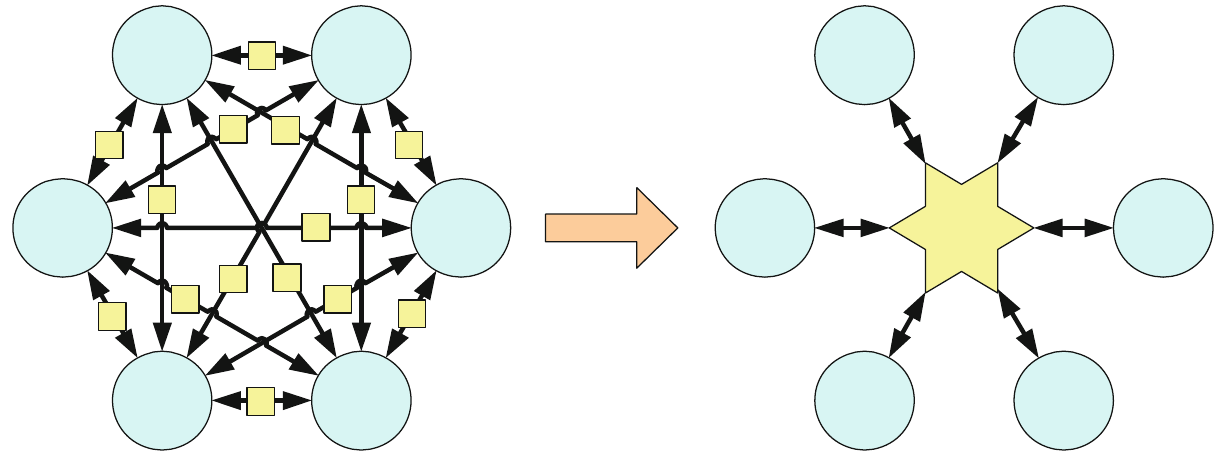
\includegraphics[width=1\textwidth]{chapters/2_background/interoperability}
        \caption{Comparison of communication by point-to-point interfaces and standards.}\label{fig:interoperability}
    \end{figure}

    \noindent Health care systems and devices should implement standards to achieve interoperability. If every application stores data in its own proprietary format, many point-to-point interfaces need to be created to allow communication. The left graph of figure~\ref{fig:interoperability} illustrates this. However, if systems adhere to a common standard by which they communicate, this is avoided. On figure~\ref{fig:interoperability} the standard is indicated by the star in the middle of the right graph. The next section briefly describes standards.

        \subsubsection{Standards}\label{standards}

        When excessive diversity creates inefficiencies and affects effectiveness, standards are required~\cite{Shortliffe2014}. A hospital contains many independent units spread across primary, secondary, and tertiary care. These units use software best fit for their practice and all record different types of data. For example: the admissions system records patient diagnosis, the pharmacy records prescriptions that were handed out, and the laboratory system records test results. Inevitably, transfer of data between these units is required. 

        To coordinate multiple systems, data must be exchanged. Nowadays too many different systems exist to create point-to-point interfaces for. Standards try to resolve this issue by defining guidelines that software systems should adhere to in order to communicate data. An efficient standard requires that data is easily stored and presented towards the users of an EHR system. Also, security measures, such as authentication and access control, should be interwoven with these standards.

        The use of standards in an EHR system leads to better interoperability which in turn leads to lower development costs. Over time, the continuous addition of proprietary data structures leads to difficult to maintain software and a higher risk of critical bugs. New medical devices and software that comply to standards prevent this. However, there is currently no regulator that enforces the use of existing standards. As a result, good interoperability lies in the hands of the software vendors.

        We close this section by giving two examples of standards. First, the most commonly used set of standards is Health Level 7~\cite{HL7}. These message-based standards provide a framework for the exchange, integration, sharing, and retrieval of electronic health information. Second, DICOM is used for the communication and management of medical imaging information~\cite{Mildenberger2002}. DICOM allows the exchange of persistent objects, such as images, which is not possible with HL7 messages.

    \subsection{Usability}\label{usability}

    We define usability as follows: ``the extent to which a product can be used by specified users to achieve specified goals with effectiveness, efficiency and satisfaction in a specified context of use''~\cite{Bevan2001}. As the health care sector deploys more and more devices and software solutions, it is of importance that these are usable. In case they are, fewer medical errors are made which improves patient safety and increases the efficiency of clinicians. Systems with poor usability may have the opposite effect, increasing the amount of errors~\cite{Koppel2005}. This also leads to more paper generation as clinicians want to circumvent the poorly usable system, as mentioned in section~\ref{paper}. Mobile technology seen today features smaller screens and receives input primarily via touch. These devices ask for completely different user interface design principles. However, no research concerning mobile device usability in health care settings was found.

    Problems detected at the start of the development cycle are less resource intensive to solve. They may expose fundamental issues which would have been a lot more costly to deal with at later stages of development. Therefore, it is important to conduct usability evaluations early on in the development phase to ensure that the health systems are developed in a cost-effective manner that results in an efficient, effective, and useful product~\cite{Edwards2008}. Usability is difficult to evaluate in the health care sector, due to the specific needs that many different work environments require. By providing customization options, each care setting may tailor the system to their wishes. However, this kind of flexibility may create other usability issues.

    Several methods exist to evaluate usability. An expert review is an example of such a method in which an expert evaluates the usability. A heuristic evaluation is similar in this regard as it consists of several experts evaluating a system. However, this method tests a system against a set of predefined usability heuristics. To give an example, Jakob Nielsen created 10 usability heuristics that are still widely used today~\cite{Nielsen1993}. The heuristics are described in appendix~\ref{appendix_nielsen}. It should be noted that expert reviews identify \emph{predicted} usability issues. To have a better chance of identifying issues that may arise during real use, an actual end user should evaluate the system. However, conducting such tests are costly in terms of time and resources, which may not be feasible. To conclude, the following list describes 14 usability principles, which are similar to Nielsen's heuristics, for the design of EHR systems~\cite{Middleton2013}:
    \begin{multicols}{2}
        \begin{myenumerate}
            \item \emph{Consistency}: design consistency and standard utilization.
            \item \emph{Visibility}: system state visibility.
            \item \emph{Match}: system and world match.
            \item \emph{Minimalism}: minimalist design.
            \item \emph{Memory}: memory load minimization.
            \item \emph{Feedback}: informative feedback
            \item \emph{Flexibility}: flexible and customizable system.
            \item \emph{Message}: useful error messages.
            \item \emph{Error}: use error prevention.
            \item \emph{Closure}: clear closure.
            \item \emph{Reversibility}: reversible actions.
            \item \emph{Language}: user language utilization.
            \item \emph{Control}: user control.
            \item \emph{Documentation}: help and documentation.
        \end{myenumerate}
    \end{multicols}

    \subsection{Telemonitoring}\label{telemonitoring}

    At the start of 21st century mobile phones were small bricks with functionality limited to calling and text messaging. Today, smartphones are used to navigate the internet, play games, watch media, and so forth. These recent technological advancements bring many new opportunities which may transform the health care industry. An example of such an opportunity is telemonitoring. Monitoring patients at a distance through the use of information technology is called telemonitoring~\cite{Field1996}. Here, the patient uses monitoring devices to gather data which in turn is sent to the health care provider. 
    
    While many health conditions can be monitored, telemonitoring is most prevalent in chronic disease management. Chronic diseases are defined as long-lasting health conditions and include the following four major types: cardiovascular disease, cancer, diabetes, and chronic obstructive pulmonary disease (COPD)~\cite{WHO2014}. Cardiovascular disease is the leading cause of death worldwide~\cite{Mendis2011}. Together with cancer, these two diseases accounted for almost half of all deaths in the United States of the year 2015~\cite{NCHS2015}. Speaking of finances, 86\% of all health care expenditure went towards patients suffering from one or more chronic conditions~\cite{Gerteis2014}. The prevention of chronic disease and improving the management thereof after onset, will yield significant benefits.
    
    These conditions often occur as a result of an unhealthy lifestyle~\cite{Willett2006}. Therefore, it is very important to spread awareness on healthy habits. Suggestions often include the following: avoid smoking, maintain a healthy weight, exercise daily and limit the time spent sedentary, and maintain a healthy diet. These lifestyle changes become even more important during chronic disease management.

    The management of chronic diseases may benefit greatly from telemonitoring. Patients have access to care while having the comfort of their homes. As a result, the patient saves time and costs associated with consultations. Relatives of the patient may also be more at ease as they know the caregiver is monitoring the situation. On the other end, health care institutions save resources as care is delivered without having the patient visit~\cite{Meystre2005}.

    At its core, telemonitoring relies heavily on interoperability as it has the potential to add many different devices to the health care infrastructure. The caregiver should be able to receive, read, and react to this data. Interoperability should already be accounted for in case the device was specifically engineered for the health care sector. However, a smartphone for example, is built for general use and not necessarily for health care. As such, these devices rely mainly on software and other connected devices to allow telemonitoring. On the other hand, extra attention must be given to usability as the telemonitoring devices often have small-sized screens. Good user interface design will lead to higher user satisfaction and may therefore impact the patient's adherence towards the management process.

    \subsection{Privacy \& security}\label{privacy}

    Privacy refers to the desire of a person to control the disclosure of personal health and other information~\cite{Shortliffe2014}. On the other hand, confidentiality is the ability to control the release of personal health information to a care provider under the agreement that the information will not be spread or used further. Security is the protection of privacy and security, which is achieved through policies, procedures, and safeguards. 

    We can ask several questions related to health information data access and storage: who owns the data? Is it the health provider or the patient? Who can read data? Who can write data? Can someone access specific health information without consent? In order to deal with the some of the challenges concerning data access and storage, these questions need to be answered~\cite{Meingast2006}.

    Medical data access raises several privacy concerns. For example, the research of the medical data of a large population may uncover looming threats or an epidemic. However, this is only possible if researchers have free access to this data, as it is not feasible to ask every individual of a population for consent. However, medical data should not be too accessible. As more and more people gain access to health data of the population, the chance of data misuse or unauthorized access increases. Therefore, striking a balance between free information access and protection of privacy and confidentiality is difficult. An argument that promotes free access is to anonymize the data by removing identifiers such as the person's name. However, the individual pieces of information can still reveal the their identity.

    Compared to paper, access to digital repositories of health records is easier. This calls for extra security measures to prevent unauthorized access. To gain access to certain records, clinicians are required to authenticate themselves. Also, access control should be present. This security technique limits access to certain data based on the privileges associated with the authenticated user. Whether the authentication succeeds or not, the audit system will always record the attempt. Such systems need clear rules and policies defined by the institution on who can access what. Data encryption is mandatory, which makes the data unreadable should data breaches ever occur.

    To further prevent malicious use of health data, institutions should educate their staff to make them aware of the privacy rules and policies that are in place. Appropriate punishments should be in place should someone violate these rules.\bigskip

    \noindent This concludes the literature overview on the electronic health record. A lot of information was presented during this chapter. Given this information, we can now design an application to resolve several issues surrounding this topic, which is the focus of the next chapter.